\section{BranchyNet}


One may argue, that the two datasets used for benchmarking are not applicable to real-life scenarios, as the images are only 32x32 pixels and the datasets only contain 10.000 samples.



This thesis studies BranchyNet on state-of-the-art \gls{dnn} ResNet50 fo image size 224x224 images, only modified to accommodate early exiting of the BranchyNet framework. ResNet50 is built up of 50 layers divided into 4 blocks. Table \ref{tbl:resnet50} describes the block and layers of the ResNet architecture. 

\pagebreak
    \begin{longtabu}{>{\bfseries}X|X[c]|X[4c]}
		\caption[ResNet50 description]{ResNet50 description. The table describes the blocks of ResNet50, the size of the block and the layers of the block.} \label{tbl:resnet50} \\
		\toprule
		\rowfont{\bfseries}
		Block name & Output size & Layer description \tabularnewline
		\hline
		\endfirsthead
		\multicolumn{3}{@{}l}{\textbf{\textcolor{black}{Table \ref{tbl:resnet50}:}} continued}\\
		\toprule
		\rowfont{\bfseries}
		Layer name & Output size & Layer description \tabularnewline
		\hline
		\endhead % all the lines above this will be repeated on every page
		\hline
		\multicolumn{3}{@{}l}{continued \ldots}\\
		\endfoot
		\hline
		\endlastfoot
		conv1 & $112\times 112$& $7\times 7, 64, \:\mathrm{stride}\: 2$ \tabularnewline \hline
		
		\multirow{5}{*}{conv2\_x} 	& \multirow{5}{*}{$56 \times 56$} 	& $3 \times 3 \:\mathrm{maxpool, stride}\: 2 $ \\ \tabucline{3-3} & & \multirow{4}{*}{
			$\begin{bmatrix}
						1 \times 1, 64 \\ 3 \times 3, 64 \\1 \times 1, 256
			 \end{bmatrix} \times 3$ }		\tabularnewline										
		& & 	\tabularnewline
		& & 	\tabularnewline
		& & 	\tabularnewline
		\hline
		
		\multirow{4}{*}{conv3\_x} 	& \multirow{4}{*}{$28\times 28$} & \multirow{4}{*}{
			$\begin{bmatrix}
			1 \times 1, 128 \\ 3 \times 3, 128 \\1 \times 1, 512
			\end{bmatrix} \times 4$ }		\tabularnewline										
		& & 	\tabularnewline
		& & 	\tabularnewline
		& & 	\tabularnewline
		\hline
		
		\multirow{4}{*}{conv4\_x} 	& \multirow{4}{*}{$14\times 14$} & \multirow{4}{*}{
			$\begin{bmatrix}
			1 \times 1, 256 \\ 3 \times 3, 256 \\1 \times 1, 1024
			\end{bmatrix} \times 6$}		\tabularnewline										
		& & 	\tabularnewline
		& & 	\tabularnewline
		& & 	\tabularnewline
		\hline
		
		\multirow{4}{*}{conv5\_x} 	& \multirow{4}{*}{$7\times 7$} & \multirow{4}{*}{
			$\begin{bmatrix}
			1 \times 1, 512 \\ 3 \times 3, 512 \\1 \times 1, 2048
			\end{bmatrix} \times 3$}		\tabularnewline										
		& & 	\tabularnewline
		& & 	\tabularnewline
		& & 	\tabularnewline
		\hline
		
		Classifier & \multicolumn2{c}{Avg. Pool, 1000-d fc, Softmax} \tabularnewline
		\bottomrule
	\end{longtabu}
	\vspace{-20pt} \textit{Source: \citetitle{he_deep_2015}, by \citeauthor{he_deep_2015} \cite{he_deep_2015}, describes a full list of Residual Networks (ResNet18, ResNet34, ResNet50, Resnet101 and ResNet152)}


The Branchy-ResNet50 makes use of the blocks defined by table \ref{tbl:resnet50} as placement for early exiting points. After each block, the intermediate features are fed to a pooling-layer and a fully-connected classifier. The prediction results are stored and the networks intermediate features are further processed until the end of the original network. Figure \ref{fig:b-resnet} visualizes the early exiting model B-ResNet50.

\begin{figure}
	\centering
	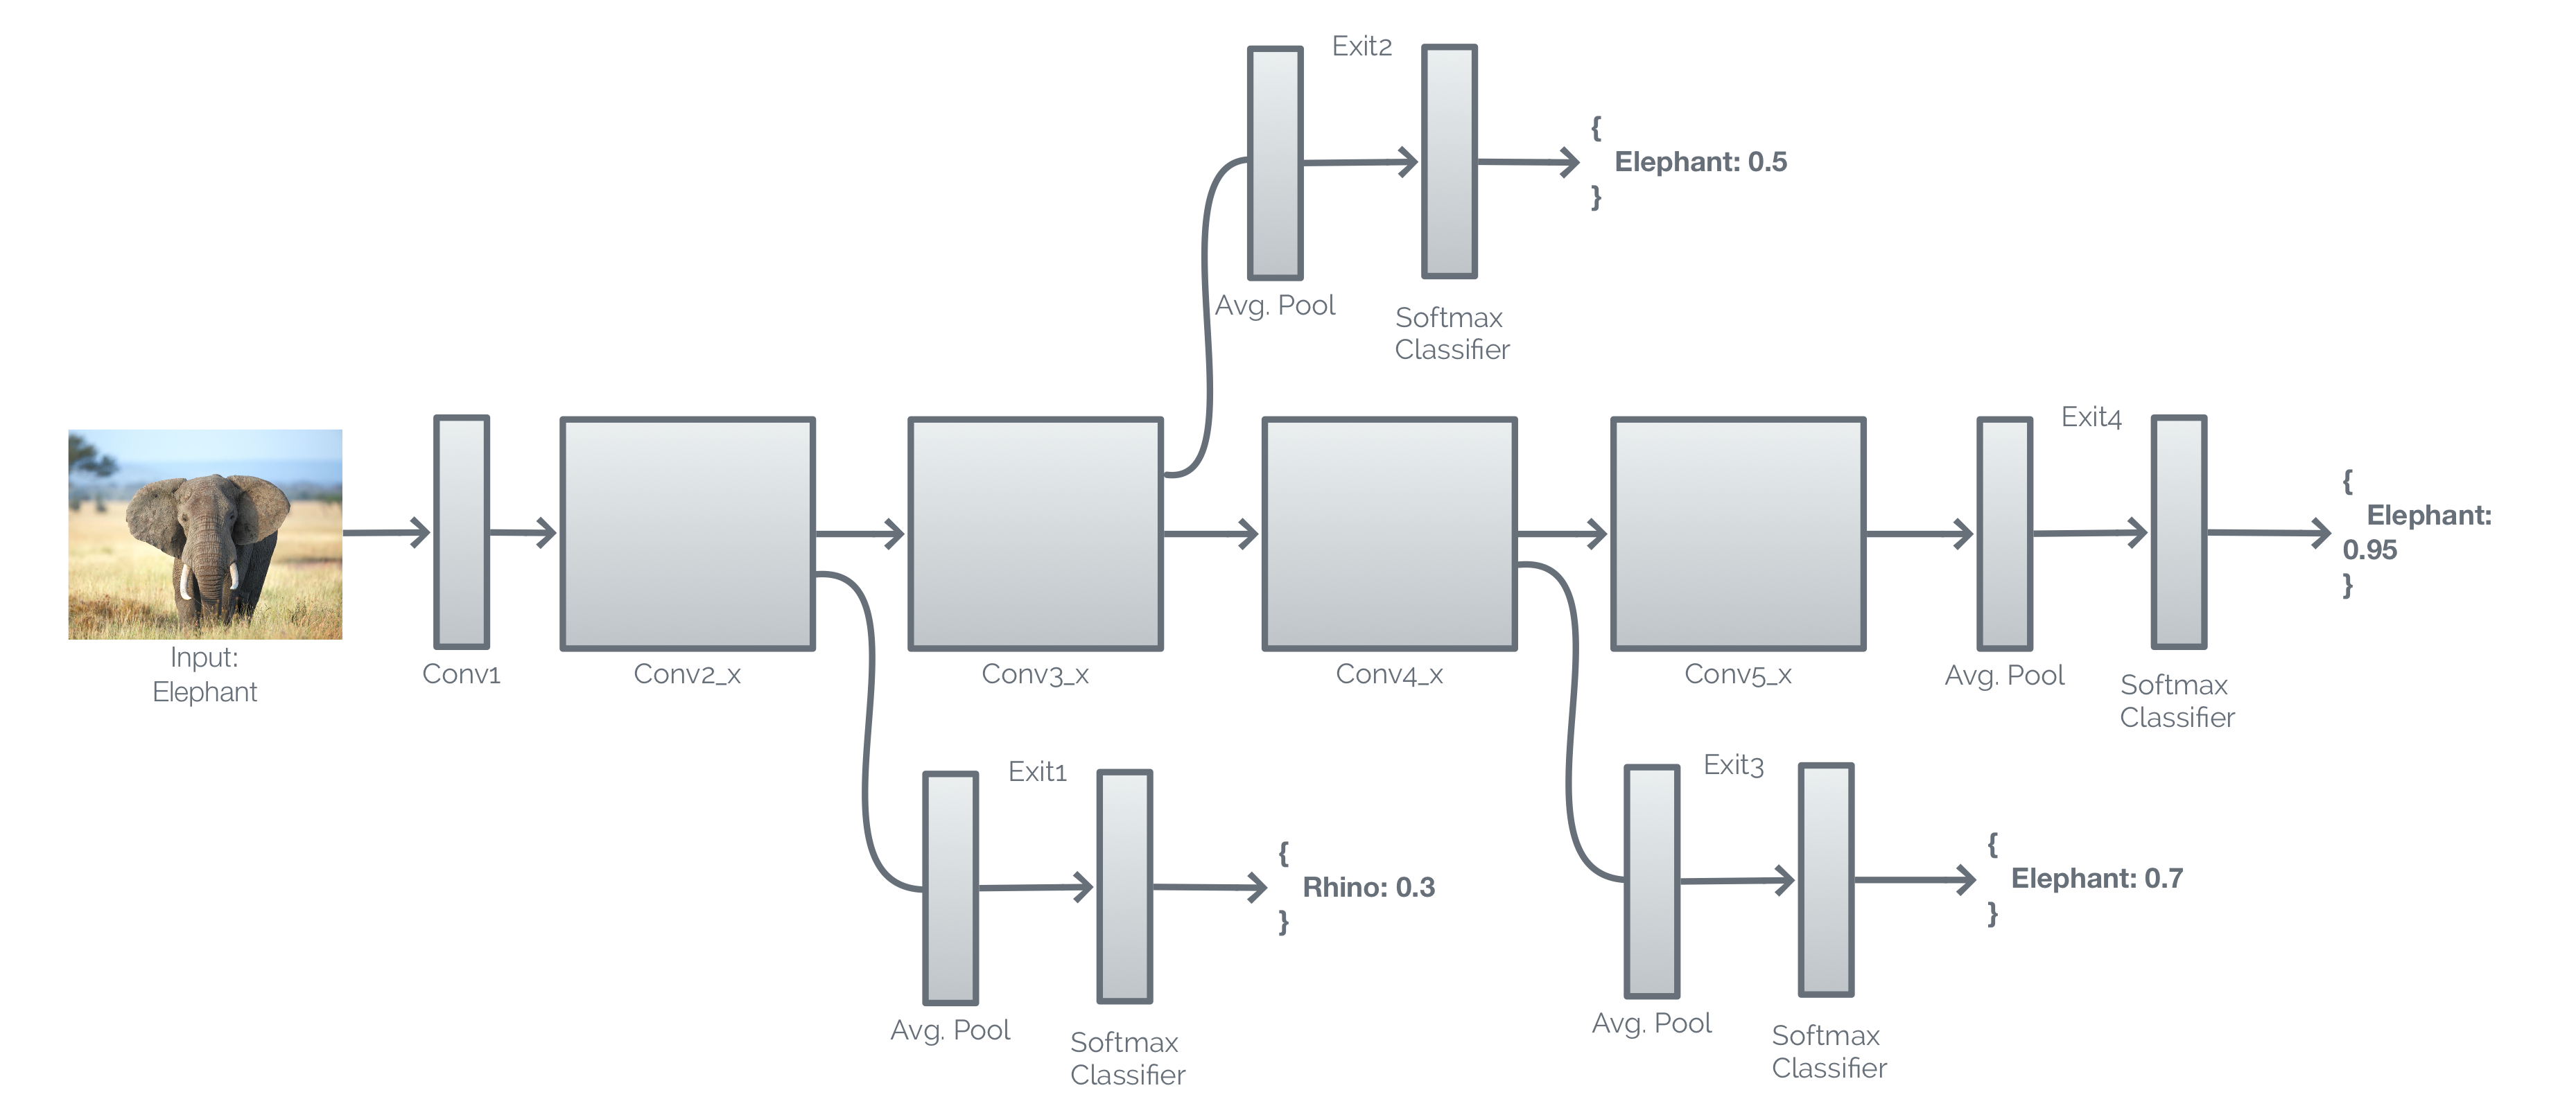
\includegraphics[width=\linewidth]{figures/models/BResNet}
	\caption[B-ResNet architecture]{Branchy-ResNet50: ResNet50 extended to implement the BranchyNet framework. The figure illustrates how classification confidence grows, as we go deeper in the model. The first exit actually fails to classify the elephant. }
	\label{fig:b-resnet}
\end{figure}



\paragraph{BranchyNet Training Framework}

The network is trained solving the joint-optimization problem is defined as the weighted sum of each branch-prediction.

\begin{align*}
	L(\hat{\mathbf{y}},\mathbf{y};\theta) = \sum_{n=1}^{N} w_m L(\hat{\mathbf{y}}_{exit_n},\mathbf{y};\theta)
\end{align*}

Where the loss function is the softmax cross-entropy objective.
The weighted sum loss is back-propagated to optimize the weights of the network. 